\documentclass[10pt]{article}

\pagestyle{empty}

\setlength{\textheight}{250mm}
\setlength{\textwidth}{180mm}
\setlength{\oddsidemargin}{-8mm}
\setlength{\topmargin}{-1.5cm}

\usepackage{amsmath}
\usepackage{amsthm}
\usepackage{psfrag}
\usepackage{graphicx}
\usepackage{bm}
\usepackage{mathrsfs}
\usepackage{icomma} % pacchetto per limitare lo spazio standard posto dopo la virgola in caso che la virgola sia tra cifre
\usepackage{amsfonts} % amplia i caratteri matematici disponibili
\usepackage{amssymb}
%\usepackage{wrapfig}
\usepackage{empheq}

\usepackage{epstopdf}
\usepackage[utf8x]{inputenc}
\usepackage{ifthen}

\usepackage[italian]{babel}
%\usepackage[latin1]{inputenc}

%\include{def}

%\newcommand{\kg}{\textrm{kg}}
%\newcommand{\K}{\textrm{K}}
%\newcommand{\m} {\textrm{m}}
%\newcommand{\dm}{\textrm{dm}}
%\newcommand{\cm}{\textrm{cm}}
%\newcommand{\mm}{\textrm{mm}}
%\newcommand{\s} {\textrm{s}}
%\newcommand{\N} {\textrm{N}}
%\renewcommand{\Pa}{\textrm{Pa}}
%\newtheorem{exerciseS}{Esercizio}
\def \flagSect{0} % 1    : numerazione
		  % else : niente
%\newcommand{\taitol}[1]  % stile titolo
%{
%%{\textit{#1}}
%{#1}
%}
\def \soluzione{Soluzione}
\def \partePrima{Concetti. }
\def \parteSeconda{Svolgimento. }
%\def \parteTerza{}
\newcommand{\sol}{\subsubsection*{\soluzione}}
\newcommand{\partone}{\ \ \ \ \ \textbf{\partePrima}}
\newcommand{\parttwo}{\vspace{0.2cm}\textbf{\parteSeconda}}

\ifnum\flagSect=1
\newtheorem{esercizio}{Esercizio}%[section]
\else
\newtheorem*{esercizio}{Esercizio}
\fi

\newtheorem*{teorema}{Teorema}
\newtheorem*{lemma}{Lemma}

% ###########################################################
%\def \flagSect{0} % 1    : numerazione
		  % else : niente
%\newcommand{\taitol}[1]  % stile titolo
%{
%%{\textit{#1}}
%{#1}
%}
\def \soluzione{Soluzione}
\def \partePrima{Concetti. }
\def \parteSeconda{Svolgimento. }
%\def \parteTerza{}
\newcommand{\sol}{\subsubsection*{\soluzione}}
\newcommand{\partone}{\ \ \ \ \ \textbf{\partePrima}}
\newcommand{\parttwo}{\vspace{0.2cm}\textbf{\parteSeconda}}

\ifnum\flagSect=1
\newtheorem{esercizio}{Esercizio}%[section]
\else
\newtheorem*{esercizio}{Esercizio}
\fi

\newtheorem*{teorema}{Teorema}
\newtheorem*{lemma}{Lemma}

% ###########################################################
%\def \flagSect{0} % 1    : numerazione
		  % else : niente
%\newcommand{\taitol}[1]  % stile titolo
%{
%%{\textit{#1}}
%{#1}
%}
\def \soluzione{Soluzione}
\def \partePrima{Concetti. }
\def \parteSeconda{Svolgimento. }
%\def \parteTerza{}
\newcommand{\sol}{\subsubsection*{\soluzione}}
\newcommand{\partone}{\ \ \ \ \ \textbf{\partePrima}}
\newcommand{\parttwo}{\vspace{0.2cm}\textbf{\parteSeconda}}

\ifnum\flagSect=1
\newtheorem{esercizio}{Esercizio}%[section]
\else
\newtheorem*{esercizio}{Esercizio}
\fi

\newtheorem*{teorema}{Teorema}
\newtheorem*{lemma}{Lemma}

% ###########################################################
%\input{logicNumb}
%\newcommand{\sectionIf}[2]
%{
%   \ifthenelse{\equal{#1}{1}}
%              {\subsection{#2}}{\subsection*{#2}}
%}
% ###########################################################

%\newcommand{\sectionIf}[2]
%{
%   \ifthenelse{\equal{#1}{1}}
%              {\subsection{#2}}{\subsection*{#2}}
%}
% ###########################################################

%\newcommand{\sectionIf}[2]
%{
%   \ifthenelse{\equal{#1}{1}}
%              {\subsection{#2}}{\subsection*{#2}}
%}
% ###########################################################



\begin{document}

\begin{center}
\textbf{Esercizi per il corso di Fluidodinamica} 
\medskip
\end{center}


\noindent
\begin{tabular}{cc}
\begin{minipage}{0.60\textwidth}
\begin{exerciseS}[Corrente di Taylor-Couette: coppia sui cilindri]
Si consideri la corrente piana di un fluido di densità $\rho$ fra due cilindri coassiali di raggio $R_1$ e $R_2$. Il cilindro esterno è fermo, mentre quello interno è messo in rotazione da un motore con curva caratteristica $C_{disp}(\Omega) = \alpha - \beta \Omega$.
Si determini il punto di equilibrio del sistema ($\Omega$ costante).
 
(\dots)
\end{exerciseS}
\end{minipage}
&
\begin{minipage}{0.35\textwidth}
   \begin{center}
   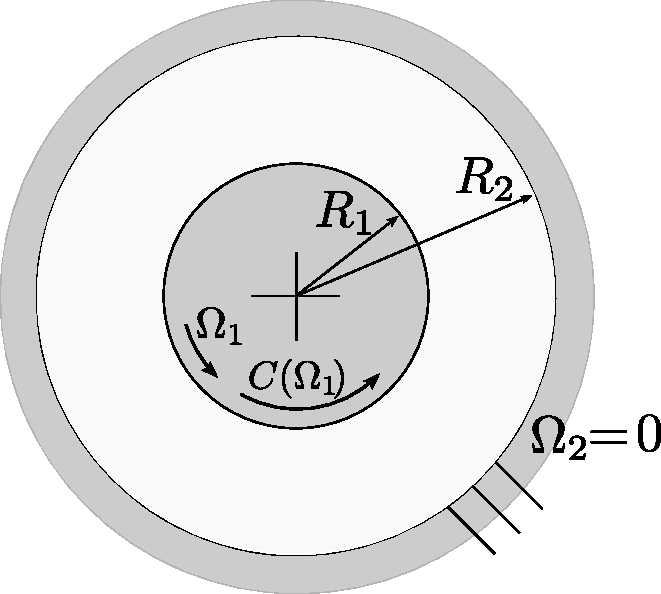
\includegraphics[width=0.95\textwidth]{./fig/slnEsatte-taylor-couette}
   \end{center}
\end{minipage}
\end{tabular}

\sol

\partone Soluzione esatte delle equazioni di Navier-Stokes in geometria cilindrica. Corrente di Taylor-Couette.

\begin{equation}
  \begin{cases}
    \rho \dfrac{\partial u_r}{\partial t}
    + \rho \left( \bm{u} \cdot \bm{\nabla}u_r - \dfrac{u_\theta^2}{r} \right)
    - \mu \left(\nabla^2 u_r 
       - \dfrac{u_r}{r^2} 
       - \dfrac{2}{r^2}\dfrac{\partial u_\theta}{\partial \theta} \right)  
       + \dfrac{\partial p}{\partial r} = f_r \\
    \rho \dfrac{\partial u_\theta}{\partial t}
    + \rho \left( \bm{u} \cdot \bm{\nabla} u_\theta + \dfrac{u_\theta u_r}{r} \right)
    - \mu \left(\nabla^2 u_\theta 
       - \dfrac{u_\theta}{r^2} 
       + \frac{2}{r^2}\dfrac{\partial u_r}{\partial \theta}  \right) 
    + \dfrac{1}{r} \frac{\partial p}{\partial \theta} = f_\theta\\
    \rho \dfrac{\partial u_z}{\partial t}
    + \rho \bm{u} \cdot \bm{\nabla} u_z
    - \mu \nabla^2 u_z
    + \dfrac{\partial p}{\partial z} = f_z \\ \\
    \dfrac{1}{r}\dfrac{\partial}{\partial r}\left( r u_r \right) 
    + \dfrac{1}{r}\dfrac{\partial u_\theta}{\partial \theta} 
    + \dfrac{\partial u_z}{\partial z} = 0
  \end{cases}
  \end{equation}
  con 
  \begin{equation}
  \begin{aligned}
  & \bm{a} \cdot \bm{\nabla} b = a_r \dfrac{\partial b}{\partial r} 
     + \dfrac{a_\theta}{r} \dfrac{\partial b}{\partial \theta}  
     + a_z \dfrac{\partial b}{\partial z} \\
  & \nabla^2 f = \dfrac{1}{r}\dfrac{\partial}{\partial r}
                      \left(r \frac{\partial f}{\partial r} \right) +
               \frac{1}{r^2} \frac{\partial^2 f}{\partial \theta^2} + 
               \frac{\partial^2 f}{\partial z^2} 
  \end{aligned}
  \end{equation}
  
\vspace{0.5cm}
Espressione vettoriale del contributo viscoso del vettore sforzo,
\begin{equation}
\begin{aligned}
  \bm{s_n} & = \mathbb{S} \cdot \bm{\hat{n}} = \\
           & = \mu [\bm{\nabla} \bm{u} + \bm{\nabla}^T \bm{u}] \cdot \bm{\hat{n}} = \\
           & = \mu \left[ 2 (\bm{\hat{n}} \cdot \bm{\nabla} ) \bm{u} + \bm{\hat{n}} \times \bm{\nabla} \times \bm{u}  \right]
\end{aligned}
\end{equation}

\parttwo Viene risolto il problema piano, nel quale i campi di velocità e di pressione hanno la forma 
\begin{equation}
 \bm{u}(\bm{r}) = u_r(r,\theta) \bm{\hat{r}} + u_{\theta}(r,\theta) \bm{\hat{\theta}} \quad , \quad P(\bm{r}) = P(r,\theta) \ ,
\end{equation}
e le azioni integrali (come la coppia fornita e quella incognita) sono intese per unità di lunghezza, essendo la ``dimensione mancante'' quella fuori dal piano del disegno.

\begin{itemize}

\item Calcolo delle velocità angolari dei cilindri. Nota la forma del campo di moto e
le velocità in due punti a diversi raggi, è possibile calcolare $\Omega_1$, $\Omega_2$
 risolvendo un sistema lineare di due equazioni nelle due incognite.
%
Il campo di moto tra due cilindri coassiali rotanti è:
\begin{equation}
  u_\theta(r) = A r + \dfrac{B}{r} = \frac{\Omega_2 R_2^2 - \Omega_1 R_1^2}{R_2^2-R_1^2} r +
   \frac{(\Omega_1 - \Omega_2)R_1^2 R_2^2}{R_2^2-R_1^2}\frac{1}{r} \ .
\end{equation}
Se il cilindro esterno è fermo e la velocità angolare del cilindro interno vale $\Omega_1 = \Omega$, i coefficienti $A$ e $B$ valgono
\begin{equation}
 A = - \frac{R_1^2}{R_2^2-R_1^2} \Omega  < 0 \qquad , \qquad B = \frac{R_1^2 R_2^2}{R_2^2-R_1^2} \Omega > 0 \ .	
\end{equation}
%
\begin{remark} La soluzione esatta di Taylor-Couette è facile da ricavare, se si ricorda
che è la somma di una rotazione rigida e un vortice irrotazionale: imponendo la forma
$u_\theta (r) = A r + B/r$ e le condizioni al contorno,
\begin{equation}
 u_{\theta}(R_1) = \Omega_1 R_1 \qquad , \qquad  u_{\theta}(R_2) = \Omega_2 R_2
\end{equation}
si ottiene la formula voluta.
\end{remark}

\item Calcolo dello sforzo tangenziale a parete per determinare il puto di equilibrio del sistema. Si determina la componente tangenziale (quella che contribuisce alla coppia resistente)
dello sforzo sul cilindro interno.
Il contributo viscoso del vettore sforzo può essere scritto come:
\begin{equation}
\begin{aligned}
  \bm{s_n} & = \mathbb{S} \cdot \bm{\hat{n}} = \\
           & = \mu [\bm{\nabla} \bm{u} + \bm{\nabla}^T \bm{u}] \cdot \bm{\hat{n}} = \\
           & = \mu \left[ 2 (\bm{\hat{n}} \cdot \bm{\nabla} ) \bm{u} + \bm{\hat{n}} \times \bm{\nabla} \times \bm{u}  \right] = &  \text{(verificare con le tabelle)} \\
           & = \mu \left[ 2 \dfrac{\partial u_\theta}{\partial r} - \dfrac{1}{r} 
    \dfrac{\partial}{\partial r} (r u_\theta) \right] \bm{\hat{\theta}} = \\
           & = \mu \left[ \dfrac{\partial u_\theta}{\partial r} - \dfrac{u_\theta}{r} \right] \bm{\hat{\theta}} = &  \text{($u_\theta = A r + B / r$)}\\
           & = - 2 \mu \dfrac{B}{r^2} \bm{\hat{\theta}} 
\end{aligned}
\end{equation}
%
\begin{remark}
 La formula dello sforzo tangenziale a parete per la corrente di Taylor-Couette è $\tau_w = \mu \left[ \frac{\partial u_\theta}{\partial r} - \frac{u_\theta}{r} \right]$,
\end{remark}
%
La parte tangenziale dello sforzo a parete sul cilindro interno è quindi $\tau_w = 
2 \mu {B}/{R_1^2}$. Integrando il prodotto tra vettore sforzo e raggio $R_1$ sulla
 superficie laterale del cilindro si ottiene la coppia resistente,
\begin{equation}
\begin{aligned}
 C_{res}(\Omega) & = \int_{\theta=0}^{2\pi} \tau_w(R_1) R_1 R_1 d\theta  = \\ & = 2\pi \tau_w(R_1) R_1^2 = -4\pi \mu \dfrac{B(\Omega)}{R_1^2}R_1^2 =  -4\pi \mu  \frac{R_1^2 R_2^2}{R_2^2-R_1^2} \Omega  = - \gamma \Omega \ .
\end{aligned}
\end{equation}
 All'equilibrio, la somma della coppia disponibile e di quella resistente deve essere uguale a zero,
%
\begin{equation}
 0 = C_{disp}(\Omega) + C_{res}(\Omega) = \alpha - \beta \Omega -  \gamma \Omega \ ,
\end{equation}
%
e quindi $\Omega = \dfrac{\alpha}{\beta + \gamma}$.
%o in simboli $\gamma \Omega = \alpha - \beta \Omega$, da cui $\Omega = \alpha / (\beta + \gamma)  $.



\end{itemize}


%%%%%%%%%%%%%%%%%%%%%%%%%%%%%%%%%%%%%%%%%%%%%%%%%%%%%%%%%%%%%%%%%%

%%%%%%%%%%%%%%%%%%%%%%%%%%%%%%%%%%%%%%%%%%%%%%%%%%%%%%%%%%%%%%%%%%

%%%%%%%%%%%%%%%%%%%%%%%%%%%%%%%%%%%%%%%%%%%%%%%%%%%%%%%%%%%%%%%%%%


%%%%%%%%%%%%%%%%%%%%%%%%%%%%%%%%%%%%%%%%%%%%%%%%%%%%%%%%%%%%%%%%%%

%%%%%%%%%%%%%%%%%%%%%%%%%%%%%%%%%%%%%%%%%%%%%%%%%%%%%%%%%%%%%%%%%%
%%%%%%%%%%%%%%%%%%%%%%%%%%%%%%%%%%%%%%%%%%%%%%%%%%%%%%%%%%%%%%%%%%

\end{document}
